\documentclass[aspectratio=169]{beamer}

\usetheme{metropolis}
\usepackage{appendixnumberbeamer}

% Base colors (from metropolis theme)
\definecolor{metDarkBrown}{HTML}{604c38}
\definecolor{metDarkTeal}{HTML}{23373b}
\definecolor{metLightBrown}{HTML}{EB811B}
\definecolor{metLightGreen}{HTML}{14B03D}

 

\metroset{numbering=fraction,progressbar=frametitle}

% \setbeamercolor*{structure}{fg=blue!80!black}
\setbeamercolor*{structure}{fg=metLightGreen}

% % \definecolor{MainColour}{rgb}{0., 0.25, 0.8}
% \colorlet{MainColour}{blue!50!black}
% \colorlet{BgColour}{blue!10}
% \colorlet{BarColour}{blue!50!black}


% %\usetheme{CambridgeUS}%{Copenhagen}%{Frankfurt}%{Singapore}%{CambridgeUS}
% \usecolortheme[named=MainColour]{structure} 
% \useoutertheme[subsection=false]{miniframes}
% \useinnertheme{circles}
% %\useinnertheme[shadow=false]{rounded}
% \setbeamertemplate{blocks}[rounded][shadow=false]

% \setbeamercovered{transparent} 
% \setbeamertemplate{navigation symbols}{} %Remove navigation bar
% \setbeamertemplate{footline}[frame number] % add page number
% \setbeamercolor{postit}{fg=MainColour,bg=BgColour}
% \setbeamercolor{structure}{bg=black!10}
% %\setbeamercolor{palette primary}{use=structure,fg=red,bg=green}
% %\setbeamercolor{palette secondary}{use=structure,fg=red!75!black,bg=green}
% \setbeamercolor{palette tertiary}{use=structure,bg=BarColour,fg=white}
% %\setbeamercolor{palette quaternary}{fg=black,bg=green}
% %\setbeamercolor{normal text}{fg=black,bg=white}
% %\setbeamercolor{block title alerted}{fg=red,bg=green}
% %\setbeamercolor{block title example}{bg=black!10,fg=green}
\setbeamercolor{block body}{bg=black!5}

% \setbeamercolor{block title alerted}{bg=red!25}
% \setbeamercolor{block body alerted}{bg=red!10}

% \setbeamercolor{block title example}{bg={rgb:green,2;black,1;white,5}}
\setbeamercolor{block body example}{bg={rgb:green,2;black,1;white,20}}
\setbeamercolor{block body alerted}{bg={metLightBrown!25}}

% \setbeamertemplate{itemize item}{\color{black!10}$\blacksquare$}
\setbeamercolor{itemize item}{fg=metDarkTeal}
\setbeamercolor{itemize subitem}{fg=metDarkTeal}

\setbeamercolor{graybc}{fg=black,bg=black!10}
\newcommand{\myblock}[1]{\begin{beamercolorbox}[dp=1ex,center,rounded=true]%
  {graybc} {\large \textbf{#1}} \end{beamercolorbox}}%


\usepackage{etex} % fixes new-dimension error
\usepackage{lmodern} % fixes warnings
\usepackage{textcomp}% fixes warnings

\usepackage{graphicx,amsmath}
\usepackage{stmaryrd} % cf. interleave
%\usepackage{./macros/myisolatin1}
%\usepackage{./macros/prooftree}
\usepackage{alltt}
%\usepackage{./macros/circle}
\usepackage{listings}
\usepackage{relsize} % relative size fonts
\usepackage[normalem]{ulem} % strikethrough text (with \sout{.})
\usepackage{tikz}
\usetikzlibrary{%
  positioning
 ,patterns
 ,arrows
 ,automata
 ,calc
 ,shapes
 ,fit
 ,fadings
 ,decorations.pathreplacing
 ,plotmarks
% ,pgfplots.groupplots
 ,decorations.markings
}
% \tikzset{shorten >=1pt,node distance=2cm,on grid,auto,initial text={},inner sep=2pt}
\tikzstyle{aut}=[shorten >=1pt,node distance=2cm,on grid,auto,initial text={},inner sep=2pt]
\tikzstyle{st}=[circle,draw=black,fill=black!10,inner sep=3pt]
\tikzstyle{sst}=[rectangle,draw=none,fill=none,inner sep=3pt]
\tikzstyle{final}=[accepting]
\usepackage[normalem]{ulem} % striking out text with \sout{...}
\usepackage{xspace}

\usepackage{transparent}

% Nicer TT fonts
\usepackage[scaled=.83]{beramono}
\usepackage[T1]{fontenc}




%------ using eurosym -------------------------------------------------------
\usepackage{eurosym}
\def\inh#1{\mbox{\small\euro}_{#1}}
\def\eith#1#2{\mathopen{[}#1 \ ,#2\mathclose{]}}

%------ using xy ------------------------------------------------------------
\usepackage[all]{xy}
%\def\larrow#1#2#3{\xymatrix{ #3 & #1 \ar[l] _-{#2} }}
\def\larrow#1#2#3{\xymatrix{ #3 & #1 \ar[l] _--{#2} }}
\def\rarrow#1#2#3{\xymatrix{ #1 \ar[r]^-{#2} & #3 }}
\def\arLaw#1#2#3#4#5{
\xymatrix{
        #1      \ar@/^1pc/[rr]^-{#4} &
        #5 &
        #2      \ar@/^1pc/[ll]^-{#3}
}}
\def\arLeq#1#2#3#4{\arLaw{#1}{#2}{#3}{#4}\leq}
%------ using pstricks (rnode etc) ------------------------------------------
%\usepackage{pstricks,pst-node,pst-text,pst-3d}
%------ using color ---------------------------------------------------------
%\newrgbcolor{goldenrod}{.80392 .60784 .11373}
%\newrgbcolor{darkgoldenrod}{.5451 .39608 .03137}
%\newrgbcolor{brown}{.15 .15 .15}
%\newrgbcolor{darkolivegreen}{.33333 .41961 .18431}
\definecolor{goldenrod}{rgb}{.80392,.60784,.11373}
\definecolor{darkgoldenrod}{rgb}{.5451,.39608,.03137}
\definecolor{brown}{rgb}{.15,.15,.15}
\definecolor{darkolivegreen}{rgb}{.33333,.41961,.18431}
\definecolor{darkgreen}{rgb}{0,0.6,0}
%
%
%\def\gold#1{{\textcolor{goldenrod}{#1}}}
%\def\brw#1{{\brown #1}}
%%\def\gre#1{{\green #1}}

\def\dgold#1{{\textcolor{darkgoldenrod}{#1}}}
\def\dkb#1{\textcolor{blue}{#1}}
\def\tdkb#1{\textbf{\textcolor{darkblue}{#1}}}
\def\gre#1{\textcolor{darkolivegreen}{#1}}
\def\gry#1{\textcolor{gray}{#1}}
\def\rdb#1{\textcolor{red}{#1}}

\definecolor{myGray}{gray}{0.85}
\newcommand{\red}[1]{\textcolor{red!80!black}{#1}\xspace}
\newcommand{\blue}[1]{\textcolor{blue}{#1}\xspace}
\newcommand{\gold}[1]{\textcolor{darkgoldenrod}{#1}\xspace}
\newcommand{\gray}[1]{\textcolor{myGray}{#1}\xspace}
\def\laplace#1#2{*\txt{\mbox{ \fcolorbox{black}{myGray}{$\begin{array}{c}\mbox{#1}\\\\#2\\\\\end{array}$} }}}
\newenvironment{bluein}{\blue}{\black\hskip -2.5pt}

%------ Setting lecture info ----------------------------------------------

\newcounter{lectureID}
\stepcounter{lectureID}
\newcommand{\getLecture}{\arabic{lectureID}\xspace}
\newcommand{\setLectureBasic}[1]{
  \title{
    #1
    }
  \author{David Pereira \and Jos\'{e} Proen\c{c}a \and Eduardo Tovar}
  \institute{CISTER -- ISEP \\ Porto, Portugal \flushright\url{https://cister-labs.github.io/fvoca2122}}
  \date{FVOCA 2021/2022\\Formal Verification of Critical Applications}
}
\newcommand{\setLecture}[2]{\setcounter{lectureID}{#1}\setLectureBasic{#2}}


\newcounter{cExercise}
\newcommand{\exercise}{\stepcounter{cExercise}Ex.\,\arabic{lectureID}.\arabic{cExercise}:\xspace}
\newcommand{\exerciseBack}{\addtocounter{cExercise}{-1}}
\newcommand{\exerciseAdd}{\stepcounter{cExercise}}
\newcommand{\doExercise}[3][0mm]{\begin{exampleblock}{\exercise #2}\wrap{\rule{0pt}{#1}}#3\end{exampleblock}}
\newcommand{\doSimpleExercise}[2][0mm]{\begin{exampleblock}{}\wrap{\rule{0pt}{#1}}\structure{\textbf{\exercise} #2}\end{exampleblock}}


%------ contexts  ---------------------------------------------------------
\newcounter{prg}
\newenvironment{prg}[1]{\refstepcounter{prg}
\noindent
\textsc{\textbf{\arabic{prg}.}} \textsc{#1} } 
{\vspace{5mm}}

\newenvironment{sprg}[1]{
\noindent
\textsc{#1} }
{\vspace{3mm}}

\newcommand\blfootnote[1]{%
  \begingroup
  \renewcommand\thefootnote{}\footnote{#1}%
  \addtocounter{footnote}{-1}%
  \endgroup
}


\newtheorem{defi}{Defini\cao}[section]
\newtheorem{defi*}{Defini\cao}
\newtheorem{lema*}{Lema}
\newenvironment{lsbcom}
      {\footnotesize  \hrule ~\\ ~\\ {\bf \sc Nota:} }
      {\hrule  ~\\ ~\\  \normalsize}
      
\newenvironment{lsbcomi}
      {\footnotesize  \hrule ~\\ ~\\ {\bf \sc Note:} }
      {\hrule  ~\\ ~\\  \normalsize}
      
\newcommand{\fimdemo}{%
\raisebox{1.7mm}{\framebox[2mm]{\rule{0mm}{0mm}}}%
\hspace{-1.55mm}%
\rule{2mm}{0.5mm}%
\hspace{-0.45mm}%
\rule{0.5mm}{2mm}%
}

\newenvironment{intf}%
     {\traco}
    {\par \nopagebreak  \traco }
\newenvironment{demo}%
     {\vspace{-5mm}\noindent {\bf Prova:}}%
    {\par \nopagebreak  \noindent \fimdemo \vspace{3mm} }
\newenvironment{demoi}%
     {\vspace{-5mm}\noindent {\bf Proof:}}%
    {\par \nopagebreak  \noindent \fimdemo \vspace{3mm} }

\long\def\CUT#1{\relax}
\def\jnowarning#1{\typeout{Warning: #1 - document page [\thepage]}}

\newenvironment{slide}[1]{\begin{frame}\frametitle{#1}}{\end{frame}}
\long\def\marginproof#1#2{
\begin{slide}{Comments}
\footnotesize Proof of #1:\\\tiny#2
\end{slide}}

\long\def\margincomment#1{
\begin{slide}{Comments}
\footnotesize #1
\end{slide}}

\long\def\marginproof#1#2{\relax}
\long\def\margincomment#1{\relax}

\def\caixa#1{\medskip
  \begin{center}
  \fbox{\begin{minipage}{0.9\textwidth}\protect{#1}\end{minipage}}
  \end{center}}
  
  \def\caixam#1{\medskip
  \begin{center}
  \fbox{\begin{minipage}{0.9\textwidth}\protect{\vspace{-5mm}#1\vspace{-5mm}}\end{minipage}}
  \end{center}}
  
   \def\caixamm#1{\medskip
  \begin{center}
  \fbox{\begin{minipage}{0.9\textwidth}\protect{\vspace{-5mm}#1}\end{minipage}}
  \end{center}}

  
  \def\caixaaa#1{\medskip
  \begin{center}
  \fbox{\begin{minipage}{0.95\textwidth}\protect{#1}\end{minipage}}
  \end{center}}

\newcommand{\caixapeq}[2][0.71]{\medskip
  \fbox{\begin{minipage}{#1\textwidth}\protect{#2}\end{minipage}}}
  
  \def\caixapeqq#1{\medskip
  \fbox{\begin{minipage}{0.85\textwidth}\protect{#1}\end{minipage}}}
  
  \def\caixamin#1{
   \begin{center}
  \fbox{\begin{minipage}{0.70\textwidth}\protect{\vspace{-5mm}#1}\end{minipage}}
  \end{center}}


\def\endprf{\begin{flushright} $\Box$ \end{flushright} \vspace{3mm}}

%------ common jno, lab  ---------------------------------------------------------
%------------
\def\wider#1{~ #1 ~}
\def\altx#1#2{\mathopen{[}#1 \ ,#2\mathclose{]}}
\def\X{\end{document}}
\def\EXIT{ \bibliographystyle{plain} \bibliography{/Users/jno/share/texinputs/jno} \end{document}}
%------------
\def\fdep#1#2#3{#1 \mathbin{\stackrel{#2}{\rightarrow\/}} #3}
\def\lift#1{\stackrel.{#1}}
\newcommand{\N}{\mathbb{N}}
\newcommand{\Z}{\mathbb{Z}}
%\def\N{I\!\!N}                             % Nat numbers
%\def\Z{Z\!\!\!Z}                           % Integers
\def\real{I\!\!R}                           % Integers

\def\name#1{\makebox[15ex][l]{\emph{#1:}} &&}
\let\kons=\underline
\def\selup#1#2#3{#3^{#1}_{#2}}
\def\plus{\mathbin{\dagger}}
\def\asor{\mathbin{|}}                    % A | B
\def\enlist#1{\mathopen{[}#1\mathclose{]}} % [a,b,...z]
\def\from{\mathbin{\leftarrow}}
\def\listdef#1#2{\enlist{ ~ #1 \asor #2 \,}} % < f(x) | x <- l>
\def\into{\mathbin{\rightarrow}}
\let\seqdef=\listdef
\def\Seq#1{{#1}^{\star}}                 % X*
\def\f{\fun F}
\def\fuc#1{\mathsf {#1}}
\def\fun#1{\mathsf {#1}}
\def\g{\fun G}
\def\ff#1{\ap\f{#1}}
\def\gg#1{\ap\g{#1}}
\def\hfilleqn#1#2{\hfill$#1\arrayin{#2}$\hfill~}
\def\enset#1{\mathopen{ \{ }#1\mathclose{ \} }} % {a,b,...z}
\newcommand{\set}[1]{\left\{ #1 \right\}} % {a,b,...z}
\def\mcond#1#2#3{#1 \rightarrow #2,#3}
\def\bang{{!}}
\def\ap#1#2{#1\,#2}
\def\pow#1{\ap{{\cal P}}{(#1)}}           \def\pow#1{{\cal P}#1} % P(X) redefined
\def\unary#1#2{\def\arg{#2}\def\omisso{}\ifx\arg\omisso{\textsf{#1}}\else\ap{\textsf{#1}}{#2}\fi}
\def\card#1{\unary{card}{#1}}             % card 
\def\ker#1{\unary{ker}{#1}}  
\def\img#1{\unary{img}{#1}}
\def\st{\dot}
\def\len#1{\unary{len}{#1}}
\def\inds#1{\unary{inds}{#1}}
\def\dom#1{\unary{$\delta$}{#1}}
\def\rng#1{\unary{$\rho$}{#1}}
\let\ran=\rng
\def\issat{\mathbin\vdash}
\def\post#1{\hbox{post-}{#1}}              % post-#1
\def\pre#1{\hbox{pre-}{#1}}                % pre-#1
\def\presat{\mathbin{\issat_{pre}}}
\def\postsat{\mathbin{\issat_{post}}}
\def\laplace#1#2{*\txt{\fbox{$\begin{array}{c}\mbox{#1}\\\\#2\\\\\end{array}$}}}
\def\PF{{\cal PF}}
\def\ler#1{{\red \em [ read: #1]}}

\def\proj#1{\pi_{#1}}
%\def\deff{\stackrel{\rm def}{=}}          % Function definition symbol
\def\deff{\, :=\, }          % Function definition symbol
\def\setdef#1#2{\mathopen{\{} #1 \asor #2 \mathclose{\}}}
\def\asor{\mathbin{|}}                    % A | B
\def\p#1{\pi_{#1}}
\def\mvdep#1#2#3{#1 \mathbin{\stackrel{\rule[-.8ex]{0pt}{0pt}#2}{\rightharpoonup\hskip-1.5ex\rightharpoonup\/}} #3}
\def\gmvdep#1#2#3#4{#1 \mathbin{\stackrel{\rule[-.8ex]{0pt}{0pt}#2}{\rightharpoonup\hskip-1.5ex\rightharpoonup_{#4}\/}} #3}
\def\sshylo#1#2{\mean{~#1,#2~}}
\def\cata#1#2{\mathopen{(\!|}#1\mathclose{|\!)}_{{\fun #2}}}
\def\split#1#2{\const{#1,#2}}
\def\tuple#1{\mathopen{\langle}#1\mathclose{\rangle}} % <a,b,...z>
\def\divides{\mathbin{\setminus}}
\def\rdiv{\mathbin{\setminus}}
\def\ldiv{\mathbin{/}}
\def\true{\mathsf{true}}
\def\mean#1{\mathopen{[\![}#1\mathclose{]\!]}}
\def\false{\mathsf{false}}
\newenvironment{lcbr}{\left\{\begin{array}{l}}{\end{array}\right.}
\def\rcb#1#2#3#4{\def\nothing{}\def\range{#3}\mathopen{\langle}#1 \ #2 \ \ifx\range\nothing::\else: \ #3 :\fi \ #4\mathclose{\rangle}}

\def\rcbVdm#1#2#3#4{#1 \ #2 \ � #4}
\def\deffVdm{\mathbin{\raisebox{.2em}{\tiny \ \underline{$\mathchar"3234$} \ }}}
\def\mapVdm#1#2{#1 \mathbin{\tilde{\rightarrow}} #2}

\def\const#1{\mathopen{\langle}#1\mathclose{\rangle}} % <a,b,...z>
\def\comp{\mathbin{\cdot}}
\def\implied{\mathbin\Leftarrow}
\def\implies{\mathbin{\Rightarrow}}
\def\arrayin#1{\begin{array}{rcl}#1\end{array}}
\def\xarrayin#1{\begin{array}{cccccc}#1\end{array}}
\def\aspas#1{``#1''}
\def\ap#1#2{#1\,#2}
\def\unary#1#2{\def\arg{#2}\def\omisso{}\ifx\arg\omisso{\textsf{#1}}\else\ap{\textsf{#1}}{#2}\fi}
\def\card#1{\unary{card}{#1}}             % card x
\def\ker#1{\unary{ker}{#1}}  
\def\img#1{\unary{img}{#1}}
\def\ijust#1#2{&#1& \rule{2em}{0pt}  \{ \mbox{\rule[-.5em]{0pt}{1.2em} \footnotesize #2 \/} \}  \nonumber\\ && }
\def\just#1#2{\\\ijust{#1}{#2}}

\def\crflx#1{\Phi_{#1}}
\def\qcomp{\mathbin\bullet}
\def\xlarrow#1#2#3{\larrow{#3}{#2}{#1}} 
%\def\equiv{\Leftrightarrow}
\def\longlarrow#1#2#3{\xymatrix{ #3 && #1 \ar[ll] _-{#2} }}
%------------

%------  lsb  ---------------------------------------------------------

\def\drawit{\nccurve[angleA=-30,angleB=-150]{->}{NA}{NB}}

\def\cnext#1{\Circle_{#1}}
\def\clast#1{\Circle[f]_{#1}}
\def\calfut#1{\square_{#1}}

\def\mdepth#1{\mathsf{md}\, #1}

\def\always{\boxempty}
\def\eventual{\Diamond}
\def\nexts{\bigcirc}
\def\until{\mathbin{\mathcal U}}


\def\setFontSize#1{\gdef\currentFontSize{#1}\fontfamily{phv}\fontsize\currentFontSize\currentFontSize\selectfont}
\def\greybox#1{*\txt{\mbox{\fcolorbox{black}{myGray}{\mbox(40,15){#1}}}}}
\def\funbox#1{*\txt{\fcolorbox{white}{myGray}{\makebox(40,15){\black $#1$}}}}
\def\condition#1{*\txt{\fontfamily{phv}\fontsize\currentFontSize\currentFontSize\selectfont\pscirclebox[linecolor=white]{$#1$}}}
\def\checkpoint{*\txt{\pscirclebox*{}}}
\def\state{*\txt{\ovalnode[fillstyle=solid,fillcolor=red]{State}{\black Internal state}}}
\def\thing#1{$\bullet$ \rule{0pt}{.7cm} & \fcolorbox{black}{myGray}{#1}}

\def\const#1{\mathopen{\langle}#1\mathclose{\rangle}} % <a,b,...z>
\def\funbox#1{*\txt{\fcolorbox{white}{gray}{\makebox(40,15){\black $#1$}}}}
\def\pair#1{\const{#1}}
\def\bim{\fuc{B}}
%\def\abim#1{\bim\, #1}
\def\abim#1{\aapf{\bim}{#1}}
\def\bimm#1{\bim #1}
\def\iso{\cong}
\def\niso{\ncong}
\def\qcom{\mathbin{\boldsymbol{;}}}
\def\id{\fuc{id}}

\def\ainv#1{\overline{#1}}

\def\rsrt{\tau_{r}}   % right and left strength
\def\rsrtp#1{\tau_{r_{#1}}}   % right and left strength
\def\lsrt{\tau_{l}}

\def\igual{\mathbin{=}}
\def\dimp{\mathbin{\Leftrightarrow}}
\def\imp{\mathbin{\Rightarrow}}
\def\dimpp{\mathbin{\leftrightarrow}}
\def\impp{\mathbin{\rightarrow}}
\def\rimp{\mathbin{\Leftarrow}}
\def\limp{\mathbin{\multimap}}

\newcommand{\sse}{\mathbin{\, \operatorname{\textsf{iff}} \,}}
\def\e{\mathbin{\wedge}}
\def\ou{\mathbin{\vee}}

\def\aconv#1{#1^{\circ}} 
\newcommand{\fdec}[3]{#1: #2 \longrightarrow  #3}
\newcommand{\fdecf}[3]{#1: #2 \longrightarrow #3}
\newcommand{\fdef}[2]{#1\;=\; #2}

\newcommand{\adec}[3]{#1 \stackrel{#2}\longrightarrow #3}
\newcommand{\fblockf}[5]{
\begin{eqnarray*}
#1&\! \! \!: \!\! \!& #2 \longrightarrow #3\\
#1 & \! \!\! #4\, = \!\!\!& #5
\end{eqnarray*}
}

\newcommand{\sos}[3]{#3 \stackrel{#2}{\longleftarrow} #1}
\def\setcat{{\sf Set}}
\def\relcat{{\sf Rel}}
\def\parcat{{\sf Par}}
\def\predcat{{\sf Pred}}
\def\ordcat{{\sf Ord}}

\def\dois{\ensuremath{\boldsymbol{2}}}
\def\abv{\stackrel{\rm abv}{=}}
\def\sana#1{\mathopen{[\!(}#1\mathclose{)\!]}}
\def\deff{\triangleq} 
\def\pint{\mathbin{\interleave}}



% Fev 2010

\def\oculos{\mathbf{\bigcirc\!\! \frown\!\! \bigcirc}}
\def\ferramentas{\stackrel{\mathbf{\doublecap}}{\bigbox\!\!\bigbox}}
%\def\Act{\cal{N}}
\def\Act{N}

\def\vec#1{\Tilde{#1}}
\def\free#1{\textsf{free}(#1)}
\def\subs#1#2#3{\enset{#1/#2}\, #3}

\def\tim{\fuc{T}}
\def\att{\fuc{at}}
\def\md{\fuc{m}}

\def\bh#1#2{\apf{\ana{#1}}{#2}}

\def\apf#1#2{#1\; #2}                   % func applic no () -- f a
\def\appf#1#2{(#1\; #2)}                   % func applic with () -- (f a)
\def\aapf#1#2{#1 #2}                   % func applic no () -- f a

\def\aappf#1#2{(#1 #2)}                   % func applic with () -- (f a)
\def\appff#1#2{#1 (#2)}                   % func applic with () -- f(a)
%\def\ana#1#2{\mathopen{[\!(}#1\mathclose{)\!]}_{#2}}
%\def\ana#1#2{\mathopen{[\!(}#1\mathclose{)\!]}_{\fun #2}}
\def\ana#1{\mathopen{[\!(}#1\mathclose{)\!]}}
\def\sana#1{\mathopen{[\!(}#1\mathclose{)\!]}}

\def\iid#1{\id_{#1}}                     %  identitade default
\def\id{\mathbin{\fuc{id}}}    

\def\atim#1{\aapf{\tim}{#1}}
\def\final#1{\omega_{#1}}
\def\initial#1{\alpha_{#1}}

\def\ialg#1{\mu_{#1}}
\def\fcoalg#1{\nu_{#1}}
\def\hdd{\fun{hd}}
\def\tll{\fun{tl}}
\def\mrg{\fun{merge}}
\def\gnn{\fun{rep}}
\def\diag{\vartriangle}
\def\codiag{\triangledown}
\def\twist{\fun{twist}}
\def\swap{\fuc{s}}
\def\rtran#1{\stackrel{#1}{\longrightarrow}}
\def\rtrant#1{\stackrel{#1}{\longrightarrow}^{\raisebox{-4pt}{\scriptsize $*$}}}
\def\tran#1{\stackrel{#1}{\longrightarrow}}
\def\primertran#1{\stackrel{#1}{\longrightarrow'}}
\def\rra{\longrightarrow}
\def\dda{{\downarrow}}
\def\ppow{\ensuremath{\mathcal{P}}} 
\def\nx{\fun{next}}
\def\utran#1{\stackrel{#1}{\longrightarrow}}  % - a - > 
\def\reach#1{\stackrel{#1}{\longrightarrow}^*}

\newcommand{\blk}[1]{\mathbb{#1}}
\newcommand{\ger}[1]{\mathfrak{#1}}

\def\vs{\emph{vs}}
\def\ie{\emph{i.e.}}
\def\cf{\emph{cf.}}

\def\eg{\emph{e.g.}}

\def\PP{\blk{P}}

%------ CCS          -----------------------------------------%
\def\ppe{\mathbin{\vartriangleright}}
\def\kcomp{\mathbin{\boldsymbol{\bullet}}}
%\def\qcomp{\mathbin{\boldsymbol{;}}}
\def\ssp{\textsc{skip}}
\def\fim{\dagger}
%\def\ppe{\gg}
\def\cnil{\mathbf{0}}
\def\cpf#1#2{#1 . #2}                           % a.P
\def\cou#1#2{#1 \mathbin{+} #2}                 % P + Q
%\def\crt#1#2{\mathbin{#1 \setminus_{#2}}}       % P \ A
%\def\crtt#1#2{\mathbin{#1 \setminus\!\setminus_{#2}}}       % P \ A
%\def\crt#1#2{\mathsf{new}\, #2\;  #1}       % P \ A
\def\crt#1#2{#1 \backslash #2}       % P \ A
%\def\crn#1#2{\{#2\}\, #1}                  % P[f]

\def\crn#1#2{\mathbin{#1[#2]}}                  % P[f]
\def\couit#1#2{\Sigma_{#1}#2}                  %  + i=1,n
\def\cpar#1#2{#1 \mid #2}                       %  |
\def\ctpar#1#2{#1 \parallel #2}                       %  |
\def\cpars#1#2#3{#1 \mid_{#3} #2}               %  |S
\def\ffix#1#2{\underline{fix}~(#1\, =\, #2)}  % fix X
\def\fffix#1#2#3{\underline{fix}_{#1}~(#2\, =\, #3)}  % fix X
\def\tfix#1#2{\underline{\Tilde{fix}}~(\Tilde{#1}\, =\, \Tilde{#2})}  % fix X
%\def\ainv#1{\Bar{#1}}                   % ~ a
\def\ainv#1{\overline{#1}}                   % ~ a
\def\cif#1#2{\fuc{if}\, #1\, \fuc{then}\, #2}
\def\ccif#1#2#3{\fuc{if}\, #1\, \fuc{then}\, #2\, \fuc{else}\, #3}

\def\fres#1#2{#1 \restriction #2}                

\def\mean#1{\mathopen{[\![}#1\mathclose{]\!]}}
\def\llbracket{\mathopen{[\![}}
\def\rrbracket{\mathopen{]\!]}}

\def\cfree#1{\fuc{fn} (#1)}
\def\cbound#1{\fuc{bn} (#1)}
\def\anew#1{\overline{#1}\mathsf{new}\, } 
\def\transitatau{\rtran{\tau}}
\def\transitaa{\rtran{a}}


\def\cHat#1{{\cal T}(#1)}
\def\free#1{\textsf{free}(#1)}
\def\fuc#1{\textsf{#1}}
\def\subs#1#2#3{\enset{#1/#2}\, #3}
\def\PP{\blk{P}}
\def\PPf{\blk{P}_{\fim}}
\def\obs{\mathbin{\sim}}                     % P ~ Q
\def\nobs{\mathbin{\nsim}}                     % P ~ Q
\def\aobs{\mathbin{\approx}}                 % P ~ Q
\def\naobs{\mathbin{\not \approx}}                 % P ~ Q
\def\cobs{=}                                 % P = Q
\def\ssort#1{\blk{L}(#1)}                   % L()
\def\sysort#1{\blk{L}_s(#1)}                   % L()

\def\athen{\comp}
\def\PP{\blk{P}}

% 2015

\def\st{\mathbf{.}\,}
\def\laplace#1#2{*\txt{\mbox{ \fcolorbox{black}{myGray}{$\begin{array}{c}\mbox{#1}\\\\#2\\\\\end{array}$} }}}
\newcommand{\galois}[2]{#1\; \dashv\; #2}

\newcommand{\fddec}[3]{#1: #2 \longrightarrow  #3}

\def\mcrl{\textsf{mCRL2}}

\def\obs{\sim}
\def\eqm{\mathbin{\equiv}}                     
\def\noeqm{\mathbin{\not\!\equiv}}  
\newcommand{\flam}[2]{\lambda_{#1}\; .\; #2}
\def\existential#1#2{\exists_{#1}\;.\; #2}
\def\existencial#1#2{\exists_{#1}\;.\; #2}

\def\diam#1{\ensuremath{\langle #1 \rangle}}
\def\boxx#1{\ensuremath{[#1]}}
\def\pv#1#2{\langle #1 \rangle\, #2}
\def\nc#1#2{[#1]\, #2}
\def\pvo#1#2{\langle \! \! \! \langle #1 \rangle \! \! \! \rangle\, #2}
\def\nco#1#2{\llbracket #1 \rrbracket #2}
\def\cvg#1{\llbracket \downarrow \rrbracket #1}
\def\cvgr#1#2{\llbracket #1 \downarrow \rrbracket #2}
\def\cvgl#1#2{\llbracket \downarrow  #1 \rrbracket #2}
\def\cvglr#1#2{\llbracket \downarrow  #1 \downarrow \rrbracket #2}
\def\lfp#1#2{\mu {#1}\, .\, {#2}}
\def\lpf#1#2{\mu {#1}\, .\, {#2}}
\def\gfp#1#2{\nu {#1}\, .\, {#2}}
\def\gpf#1#2{\nu {#1}\, .\, {#2}}
\def\mset#1{\vvv #1 \vvv}
\def\vvv{\vert \! \vert}
\def\mnc#1{\vvv [#1] \vvv}
\def\mpv#1{\vvv \langle #1 \rangle \vvv}
\def\bcomp#1{#1^{\text{c}}}
\def\eqm{\mathbin{\simeq}}
\def\noeqm{\mathbin{\not\!\simeq}}
\def\universal#1#2{\forall_{#1}\; .\; #2}
\def\existential#1#2{\exists_{#1}\; .\; #2}
\def\oexistential#1#2{\exists^{1}_{#1}\; .\; #2}

\def\reach#1{\stackrel{#1}{\longrightarrow}^*}


\def\rra{\longrightarrow}

\def\Lg#1{\mathsf{Lang}(#1)}
\def\Tr#1{\mathsf{Tr}(#1)}

\def\PP{\blk{P}}

\def\paths#1{\mathsf{Paths}(#1)}
\def\Mcomma{\text{ ,}}
\def\Msemicolon{\text{ ;}}
\def\Mdot{\text{ .}}


%%%%%%%%%%%%%%%% NUNO reconf

\def\node#1{\ensuremath{\underline{#1}}}
\def\nameset{\ensuremath{\mathcal{I}}\xspace}
\def\endnameset{\ensuremath{\mathcal{E}}\xspace}
\def\nodeset{\ensuremath{\mathcal{N}}\xspace}
\def\portset{\ensuremath{\Sigma}\xspace}
\def\coordpatset{\ensuremath{\mathcal{P}}\xspace}
\def\logicmodel{\ensuremath{\mathcal{M}}\xspace}
\def\reconfset{\ensuremath{\mathcal{R}}\xspace}
\def\reconfoperationset{\ensuremath{\mathcal{O}}\xspace}
\def\channelset{\ensuremath{\mathcal{C}}\xspace}
\def\stateset{\ensuremath{\mathcal{S}}\xspace}
\def\typeset{\ensuremath{\mathcal{T}}\xspace}
\newcommand{\chanodesof}[2][\rho]{\ensuremath{\mathfrak{N}_{#1}^{#2}}\xspace}
\newcommand{\reconfop}{\ensuremath{\mathbin{\bullet}}}

\newcommand{\byreconfof}[1]{\ensuremath \stackrel{\rm #1}{\longleftarrow}}

\def\trans#1{\stackrel{#1}{\longrightarrow}}
\def\TS#1{\mathcal{G}(#1)}
\def\TSn#1{\mathcal{G}_{nodes}(#1)}


%%%%%%%%%%%%%%%%%%%%%%%%% ALEXANDRE
 \def\HHL{\mathcal{HHL}}
 
 \def\emskip{\vskip 1em}
 
 %%%%%%%%%%%%%%%%%%%%%% COMPONENTES NOV 2015
 \def\para{\mathbin{\boxtimes}}   % Mealy produto (sincrono)
\def\parc{\mathbin{\boxplus}}    % Mealy soma
\def\pars{\mathbin{\boxast}}     % Mealy misto
\def\shk#1#2{\bigl(#1\bigr)_{#2}}            % separated hook direita
\def\hk#1#2{#1\! \Lsh_{#2}}            % hook direita
\def\hkespaco#1#2{#1 \Lsh_{#2}}            % hook direita
%\def\feed#1{\Bigl( #1 \Bigr)\! \Lsh}            % hook direita
\def\feed#1{#1 \Lsh}            % hook direita
\def\kh#1#2{~_{#2}(#1)}           % hook esquerda

\def\flift#1{\ulcorner #1 \urcorner}           % funcoes embb
\def\singr#1{\lfloor #1 \rceil}

\def\pdiag{\bigtriangleup}      % diagonal em componentes
\def\pcodiag{\bigtriangledown}    % codiagonal em componentes

%\qcomp{\mathbin{\mathbf{;}}}
%\def\qcom#1#2{#1\qcomp#2}
%\def\sync{}  %d� problemas com o reotex.sty do Nuno Oliveria

 
 %%%%
 \def\SING{\ensuremath{\boldsymbol{1}}}
\def\ZERO{\ensuremath{\boldsymbol{0}}}

\def\ptran#1{\stackrel{#1}{\leadsto}}
\def\pptran#1#2{\stackrel{#1[#2]}{\leadsto}}

\def\bblue#1{\dkb{#1}}
\def\ctt#1{\underline{#1}}    
\def\lvazio{\fuc{nil}}   
\def\lcons{\mathbin{\fuc{cons}}} 
\def\either#1#2{[#1,#2]}
\def\att{\fun{at}}
\def\hd#1{\mathbin{\fuc{hd}} \, {#1}}              % hd x
\def\tl#1{\mathbin{\fuc{tl}} \, {#1}}   
\def\hdd{\mathbin{\fuc{hd}}}              % hd x
\def\tll{\mathbin{\fuc{tl}}}              % hd x\def\nnat{\blk{N}}
\def\rreal{\blk{R}}
\def\nnat{\blk{N}}
\def\vtran#1#2#3{#1\downarrow_{#3} #2 }
\def\labtran#1#2{~_{#1}\!\stackrel{#2}{\longleftarrow\, }}
\def\rabtran#1#2{\stackrel{#2}{\longrightarrow}_{#1}\, }
\def\excp#1{#1 + \SING}
\def\usplit#1#2{\langle #1, #2 \rangle}
\def\nnx{\fun{nx}}
\def\nxc{\ainv{\fun{nx}}}
%\def\ct{\fun{ct}}
%\def\ctc{\ainv{\fun{ct}}}
%\def\ini{\fun{ini}}
\def\nil{\underline{\fun{nil}}}
\def\att{\fun{at}}
\def\nx{\fun{next}}
\def\md{\fun{m}}
\def\acc{\ainv{\fun{ac}}}
\def\ac{\fun{ac}}
\newcommand{\mcar}[3]{(#1\, \rightarrow\, #2, \,   #3)}
\def\distr{\fuc{dr}}
\def\distl{\fuc{dl}}
\def\hdi#1{\mathbin{\fuc{last}} \, {#1}}              % hd x
\def\tli#1{\mathbin{\fuc{blast}} \, {#1}} 
\def\ip#1{\iota_{#1}}
\def\apf#1#2{#1\; #2}   
\def\m{\fuc{M}}

\def\onefuc{\fuc{Id}}
\def\triple#1{\const{#1}}
\def\kcomp{\mathbin{\boldsymbol{\bullet}}}  
 
\def\ntarrow{\Longrightarrow}
\newcommand{\ntdec}[3]{#1: #2 \ntarrow #3}
\def\ntiso{\stackrel{\iso}{\ntarrow}}

\def\rsrt{\tau_{r}}   % right and left strength
\def\rsrtp#1{\tau_{r_{#1}}}   % right and left strength
\def\lsrt{\tau_{l}}
\def\lsrtp#1{\tau_{l_{#1}}}   % right and left strength
\def\deltab{\delta}
\def\rpd{\delta_{r}}   % strength combination
\def\rpdp#1{\delta{r_{#1}}}
\def\lpd{\delta_{l}}
\def\ltrocam{\fuc{xl}_{+}}  % \assoc inv . \swap . \assoc
\def\rtrocam{\fuc{xr}_{+}}  
\def\dtrocam{\fuc{m}_{+}}  
\def\ltroca{\fuc{xl}}  % \assoc inv . \swap . \assoc
\def\rtroca{\fuc{xr}}  
\def\dtroca{\fuc{m}}  
\def\troca{\fuc{x}}  
\def\cat#1{{\sf #1}}
\def\flift#1{\ulcorner #1 \urcorner} 
\def\PR{\cat{Cp}}
\def\PRSp{\cat{Cp}_{Sp}}
\def\prcat#1{{\sf Cp_{#1}}}
%\newcommand{\prhom}[2]{\PR_{\bim}(#1, #2)}
\newcommand{\prhom}[2]{\PR(#1, #2)}
%\newcommand{\prhoms}[2]{\PR_{\bim}(#1, #2)_{Sp}}
\newcommand{\prhoms}[2]{\PR(#1, #2)_{Sp}}
\def\cid#1{\fuc{copy}_{#1}} 
\def\bismp#1{\sim{#1}}
\def\bism{\mathbin{\sim}}
\def\nbism{\overset{\bullet}{\sim}}
\def\nobism{\mathbin{\not\!\sim}}
\def\nilc{\fuc{nil}}
\def\idle{\fuc{idle}}
\def\inert#1{\fuc{inert}_{#1}}
\def\zerol{\fuc{zl}}
\def\zeror{\fuc{zr}}
\def\distr{\fuc{dr}}
\def\distl{\fuc{dl}}
\def\assoc{\fuc{a}}
\def\assocs{\fuc{a_*}}
\def\assocm{\fuc{a_+}}
\def\swap{\fuc{s}}
\def\swaps{\fuc{s_*}}
\def\swapm{\fuc{s_+}}
\def\lunit{\fuc{l}}
\def\runit{\fuc{r}}
\def\lunits{\fuc{l_*}}
\def\runits{\fuc{r_*}}
\def\lunitm{\fuc{l_+}}
\def\runitm{\fuc{r_+}}
\def\ana#1#2{\mathopen{[\!(}#1\mathclose{)\!]}_{#2}}
\def\sana#1{\mathopen{[\!(}#1\mathclose{)\!]}}
\def\bh#1#2{\apf{\ana{#1}}{#2}}
\def\BH{\cat{Bh}}
\def\diag{\vartriangle}
\def\codiag{\triangledown}
\def\psplit#1#2{\mathopen{\langle}#1, #2\mathclose{\rangle}}
\def\flift#1{\ulcorner #1 \urcorner} 
\def\rpdp#1{\delta{r_{#1}}}
\def\lpd{\delta_{l}}
%\def\lpdp#1{\lpd_{#1}}
\def\lpdp#1{\delta{l_{#1}}}

\def\bunit#1{\eta_{#1}}   % monad unit
\def\bmul#1{\mu_{#1}}   % monad multi

\def\bag#1{\fuc{Bag}_{#1}}

\newcommand{\MH}{\mathcal{H}}
\newcommand{\M}{M}
\newcommand{\Rz}{\textsc{T}}
\newcommand{\docircrlh}[2]{%
  \ooalign{$#1\rightarrow$\cr\hfil$#1\comp$\hfil\cr}}
\newcommand{\karrow}{\mathrel{\mathpalette\docircrlh\relax}}
\newcommand{\eqdef}{\widehat{=} \> \>}
\newcommand{\conc}{\> {\small \texttt{+} \hspace{-0.1cm} \texttt{+}} \>}
\newcommand{\mtime}{ [ 0, \infty ) }
\newcommand{\longerarrow}{\xrightarrow{\hspace*{1cm}}}
\newcommand{\klH}{\topo_{\MH}}
\newcommand{\topo}{{\bf Top}}
\def\hmul#1#2#3 { #1 \> \lhd \> #2 \> \rhd \> #3 }
\def\qcompp{\mathbin{\boldsymbol{;}}}
\def\qcom#1#2{#1\qcompp#2}


%--------------------
%--- by jose 2016 ---
%--------------------

\newcommand{\wrap}[2][]{\begin{tabular}[#1]{@{}c@{}}#2\end{tabular}}
\newcommand{\mwrap}[1]{\ensuremath{\begin{array}{@{}c@{}}#1\end{array}}}
\def\trans#1{\xrightarrow{#1}}  % - a - > 
\def\Trans#1{\stackrel{#1}{\Longrightarrow}} % =a=> 
\newcommand{\transp}[2][35]{\color{fg!#1}#2}
\newcommand{\transpt}[2][.35]{\tikz{\node[inner sep=1pt,fill opacity=0.5]{#2}}}
\newcommand{\faded}[2][0.4]{{\transparent{#1}#2}} % alternative to "transp" using transparent package

\usepackage{multicol}

\newcommand{\frsplit}[3][.48]{
  \begin{columns}%[T] % align columns
  \begin{column}{#1\textwidth} #2 \end{column} ~~~
  \begin{column}{#1\textwidth} #3 \end{column} \end{columns}
}
\newcommand{\frsplitdiff}[4]{
  \begin{columns}%[T] % align columns
  \begin{column}{#1\textwidth} #3 \end{column} ~~~
  \begin{column}{#2\textwidth} #4 \end{column} \end{columns}
}
\newcommand{\frsplitt}[3][.48]{
  \begin{columns}[T] % align columns
  \begin{column}{#1\textwidth} #2 \end{column} ~~~
  \begin{column}{#1\textwidth} #3 \end{column} \end{columns}
}
\newcommand{\col}[2][.48]{\begin{column}{#1\textwidth} #2 \end{column}}
\newcommand{\colb}[3][.48]{\begin{column}{#1\textwidth} \begin{block}{#2} #3 \end{block} \end{column}}
% rules
\newcommand{\typerule}[4][]{\ensuremath{\begin{array}[#1]{c}\textsf{\scriptsize ({#2})} \\#3 \\\hline\raisebox{-3pt}{\ensuremath{#4}}\end{array}}}
\newcommand{\styperule}[3][]{\ensuremath{\begin{array}[#1]{c} #2 \\[0.5mm]\hline\raisebox{-4pt}{\ensuremath{#3}}\end{array}}}
\newcommand{\shrk}{\vspace{-3mm}}


\newcommand{\evm}[1]{\langle #1 \rangle\,}
\newcommand{\alm}[1]{[#1]\,}

\newcommand{\mi}[1]{\ensuremath{\mathit{#1}}\xspace}
\newcommand{\mf}[1]{\ensuremath{\mathsf{#1}}\xspace}


\newcommand{\myparagraph}[1]{\medskip\noindent\textbf{#1}~~}


% Listing
\lstset{%language=Java
%  ,basicstyle=\footnotesize
  ,columns=fullflexible %space-fexible
  ,keepspaces
%  ,numberstyle=\tiny
  ,mathescape=true
  ,showstringspaces=false
%  ,morekeywords={refract,global,local,on-change}
  ,morecomment=[l]{\%}
  ,commentstyle=\sl\sffamily\color{gray}\scriptsize
  ,basicstyle=\ttfamily\relsize{-0.5}
  ,keywordstyle=\bf\color{red!50!blue}                % morekeywords={...} - not used
%  ,emphstyle=\it\sffamily\color{blue!80!black}
  ,emphstyle=\bfseries\itshape\color{blue!80!black}       % moreemph={...} - layer keywords
  ,emphstyle={[2]\itshape\color{red!70!black}}%\underbar} % moreemph={[2]...} - inner keywords
  ,stringstyle=\color{darkgreen}
  ,alsoletter={-,||,+,<>,&&,=>,|}
  ,literate=*{->}{{{\color{red!70!black}$\to$}}}{1}
             {.}{{{\color{red!70!black}.}}}{1}
             {+}{{{\color{red!70!black}+}}}{1}
             {*}{{{\color{red!70!black}*}}}{1}
             {\#}{{{\color{red!70!black}\#}}}{1}
             {&}{{{\color{red!70!black}\&}}}{1}
             {!}{{{\color{red!70!black}!}}}{1}
             {:=}{{{\color{red!70!black}:=}}}{1}
             {||}{{{\color{red!70!black}$\rule{1mm}{0mm}\|\rule{1mm}{0mm}$}}}{1}
  ,emph={act,proc,init,sort,map,var,eqn}
  ,emph={[2]block,hide,comm,rename,allow,||,<>,sum,&&,=>}
%  ,emphstyle={[2]\color{blue}}2
  ,framerule=1pt
  ,backgroundcolor=\transparent{0.02}\color{black}
  ,rulecolor=\color{black!30}
  ,frame=tblr
  ,xleftmargin=4pt
  ,xrightmargin=4pt
  ,captionpos=b
%  ,belowcaptionskip=\medskipamount
  ,aboveskip=\baselineskip
  ,floatplacement=htb
}
\lstdefinestyle{bash}{literate=*}
\newcommand{\code}[2][]{\lstinline[basicstyle=\ttfamily\relsize{-0.5},columns=fullflexible,keepspaces,#1]�#2�}
\newcommand{\mcode}[1]{\text{\code{#1}}}
\newcommand{\bash}[1]{\lstinline[basicstyle=\ttfamily\relsize{-0.5}\color{darkgreen},keywordstyle=\bf\sffamily\color{purple},columns=fullflexible,keepspaces,literate=*]�#1�}



\newcommand{\uppbox}[3][20mm]{\tikz{
  \node[black!15,fill=black!15,minimum width=#1,align=left](title){\textbf{{\footnotesize #2}}};
  \node[black!15,fill=black!15,left,xshift=4mm]at(title.east){\textbf{{\footnotesize #2}}};
  \node[blue!60!cyan,right] at(title.west){\textbf{{\footnotesize #2}}};
  \node[below,inner sep=2mm,fill=white,xshift=2mm](box)at(title.south){\includegraphics[width=#1]{#3}};
  \node[fit=(title)(box),draw=black,inner sep=0pt]{};
}}

\newcommand{\uppboxv}[3][20mm]{\tikz{
  \node[below,inner sep=2mm,fill=white](box){\includegraphics[height=#1]{#3}};
  \coordinate[yshift=5mm](top)at(box.north);
  \node[fit=(top)(box.north west)(box.north east),inner sep=0pt,fill=black!15](title){};
  \node[blue!60!cyan,right] at(title.west){\textbf{{\footnotesize #2}}};
  \node[fit=(title)(box),draw=black,inner sep=0pt]{};
}}
\usepackage{bussproofs}


\setLecture{7}{Hoare Logic and Verification Condition Generation\\\small{Continued}}

% \title{
% 	RAMDE -- Requirements and Model-driven Engineering 
% 	}
% \author{David Pereira \and Jos\'{e} Proen\c{c}a}
% \institute{CISTER -- ISEP \\ Porto, Portugal}
% \date{MScCCSE 2020/21}


\begin{document}

\frame[plain]{\titlepage}


\section{The Simple Imperative Language\\\small{With Assertions and Specifications}}

\newcommand{\kw}[1]{\structure{\text{#1}}}


\begin{slide}{Hoare Triples - review}
  
  \begin{block}{Core concept}
    The atomic concept that we will be using in order to reason about the partial correctness of programs is that known as {\em Hoare Triple}. It is a specification of the form $$\{P\}\,C\,\{Q\}$$ that reads as follows: for all states satisfying the {\em \alert{precondition}} $P$, if the program $C$ executes and terminates in a state satisfying the {\em \alert{postcondition}} $Q$, then the triple is valid.
  \end{block}
%  \begin{block}{Design by Contract}
%  These preconditions and postconditions, as well as other types of logical specifications that we will see ahead, are also known as {\em {\bf contracts}}, that is, they bound the developer to implement code that satisfies the prescribed logical specifications to ensure partial correctness.
%  \end{block}
\end{slide}

\begin{slide}{A language for Hoare Triples}
  The syntax of the language that we will be using is an extension of the basic Imperative Language with logical assertions, plus the concept of \textbf{Hoare Triple}. 
  \begin{align*}
  x &~\in~ \text{Identifiers}
  \\
  n &~\in~ \mathbb{Z}
  \\
  B &~::=~ \kw{true} ~~|~~ \kw{false}  ~~|~~ B~ \&\& B ~~|~~ B ~||~ B ~~|~~ ! B ~~|~~ E<E ~~|~~ E=E
  \tag{boolean-expr}\\
  E &~::=~ n ~~|~~ x ~~|~~ E+E ~~|~~ E*E ~~|~~ E-E
  \tag{int-expr}\\
  C &~::=~ \kw {skip} ~~|~~ C;C ~~|~~ x:=E
 ~~|~~  \kw{if } B \kw{ then } C\kw{ else }C ~~|~~  \kw{while }B\kw{ do }C
  \tag{command}\\
  A &~::=~ \kw{true} ~~|~~ \kw{false}  ~~|~~ E<E ~~|~~ E=E ~~|~~ A \land A ~~|~~ A \lor A ~~|~~ \lnot A ~~|~~ A \to A\\
  &~~~~~|~~  \forall x. A ~~|~~\exists x.A \tag{assertions}\\
  S & ~::=~ \{\alert{A}\}\;C\;\{\alert{A}\}\tag{specification/Hoare Triple}
\end{align*}
\end{slide}

\section*{Hoare Logic\\\small{Proof Rules and Verification Conditions Generation}}

%\begin{slide}{Validity of Hoare Triples}
%\begin{block}{How to check the validity of Hoare Triples?}
%  \begin{itemize}
%    \item the usual method for assuring the validity of Hoare Triples is to use a {\bf sound}
%program-proof system. 
%  \item by sound one means that it should not allow to conclude specifications that are not valid. 
%  \end{itemize}
%\end{block}
%\begin{block}{Program-Proof System}
%  A program-proof system is a set of inference rules that can be seen as fundamental laws about programs. In the next slides, we will present such rules. 
%\end{block}  
%\end{slide}

%\begin{frame}[fragile]{The Program-Proof System Rules}
%\begin{block}{The case of the \kw{skip} command}
%The \kw{skip} command does not change the state of the program. Hence, the precondition and postconditions must be the same.
%  \begin{prooftree}
%       \AxiomC{$$}
%       \UnaryInfC{$\{P\}\;\kw{skip}\;\{P\}$}
%  \end{prooftree} 
%\end{block}
%\end{frame}
%
%\begin{frame}[fragile]{The Program-Proof System Rules}
%  \begin{block}{The case of the assignment command}
%  The assignment rule states that a postcondition $Q$ can be granted for an assignment command if the condition that results from substituting $E$ for $x$ in $Q$ holds as precondition.
%  
%  %In the case of assignment, the value assigned to a variable is (possibly) changed, and thus we need to show that the precondition $P$ implies the postcondition $Q$ with the value of the variable $x$ replace by the value of the expression $E$.
%    \begin{prooftree}
%      \AxiomC{$$}
%      \UnaryInfC{$\{Q[x \mapsto E]\}\;x:=\,E\;\{Q\}$}
%    \end{prooftree}
%  \end{block}
%  \begin{block}{Instances of the above axiom}
%    \begin{itemize}
%      \item $\{Y = \kw{2}\}\;x := 2\;\{Y = \kw{X}\}$  
%      \item $\{\kw{x + 1} = n + 1\}\;x := x + 1\;\{\kw{x} = n + 1\}$    
%      \item $\{\kw{E} = E\}\;x := E\;\{\kw{x} = E\}$  
%    \end{itemize}
%
%  \end{block}
%
%\end{frame}
%
%\begin{frame}[fragile]{The Program-Proof System Rules}
%  \begin{block}{The case of command sequence}
%  When in the presence of a sequence of commands, we must prove that if the first command $C_1$ terminates in a postcondition $R$ then, the second command $C_2$, satisfying $R$ at start, if terminates, must do so in the prescribed postcondition $Q$.
%    \begin{prooftree}
%      \AxiomC{$\{P\} C_1 \{R\}$}
%      \AxiomC{$\{R\} C_2 \{Q\}$}
%      \BinaryInfC{$\{P\} C_1\,\textbf{;}\,C_2 \{Q\}$}
%    \end{prooftree}
%  \end{block}
%\end{frame}
%
%\begin{frame}{An example of the sequence rule}
%  \begin{block}{A short example}
%  By the assignment axiom we have:
%  \begin{itemize}
%  \item [(i)]$\{X = x \land Y = y\}\;R := X\;\{R=x \land Y=y\}$ 
%  \item [(ii)]$\{R = x \land Y = y\}\;X := Y\;\{R=x \land X=y\}$
%  \item [(iii)]$\{R = x \land X = y\}\;Y := R\;\{Y=x \land X=y\}$
%  \end{itemize}
%  By (i) and (ii) and the sequence rule we obtain
%  $$(iv)\:\:\{X = x \land Y = y\}\;R := X; X := Y\;\{R=x \land Y=y\}$$
%  Now, by (iv) and (iii) we finish the deduction
%  $$\{X = x \land Y = y\}\;R := X; X := Y;Y := R\;\{Y=x \land X=y\}$$
%  \end{block}
%\end{frame}
%
%
%\begin{frame}[fragile]{The Program-Proof System Rules}
%  \begin{block}{The case of conditionals}
%  In the case of conditionals, one must prove that independently of the value of the Boolean $B$ that serves as a guarda for the conditional. 
%    \begin{prooftree}
%      \AxiomC{$\{B \land P\}\,C_1\,\{Q\}$}
%      \AxiomC{$\{\neg B \land P\}\,C_2\,\{Q\}$}
%      \BinaryInfC{$\{P\}\,\kw{if}\,B\,\kw{then}\,C_1\,\kw{else}\,C_2\,\{Q\}$}
%    \end{prooftree}
%  \end{block}
%
%
%\end{frame}
%
%\begin{frame}[fragile]{The Program-Proof System Rules}
%  \begin{block}{The case fo while loops}
%  In the case of loops, we need to prove an invariant $I$ (i.e., a condition that must hold at the entry and exit of the loop) throughout all the iterations of the loop (we don't know beforehand how many will be). 
%    \begin{prooftree}
%      \AxiomC{$\{B \land I\}\,C_1\,\{I\}$}
%      \UnaryInfC{$\{I\}\,\kw{while}\;B\;\kw{do}\;C_1\{I \land \neg B\}$}
%    \end{prooftree}
%  \end{block}
%\end{frame}
%
%\begin{frame}[fragile]{The Program-Proof System Rules}
%  \begin{block}{The case of logical consequence}
%    This one is a special rule that deals only with logical assertions. It establishes a connection with first-order logic by means of side conditions that are assertions rather than specifications.     
%    \begin{prooftree}
%%      \AxiomC{$P \to P_1$}
%       \AxiomC{$\{P_1\}\,C\,\{Q_1\}$}
%%       \AxiomC{$Q_1 \to Q$}
%       \UnaryInfC{$\{P\}\,C\,\{Q\}$}     
%    \end{prooftree}
%    if $P \to P_1$ and $Q_1 \to Q$ hold (these are called side-conditions of the rule). Note also that this rule implies that Hoare logic is not meant to be used by itself; it must always be accompanied by some device for establishing the validity of side conditions, such as a decision procedure based on satisfiability, or an inference system for first-order logic.
%  \end{block}
%\end{frame}
%
%
%
%\begin{frame}[fragile]{The Program-Proof System Rules}
%  \begin{block}{A simple example using the logical consequence rule}
%  The small derivation below shows the applicability of the logical consequence rule, followed by the assignment rule. The logical consequence rule generates two side effects which can be trivially proved, and enables the application of the assignment rule.
%    \begin{prooftree}
%      \AxiomC{}
%      \RightLabel{(assignment rule)}
%      \UnaryInfC{$\{x + 1 > 10\}\;x := x + 1\;\{x > 10\}$}
%      \RightLabel{if $x > 10 \to x + 1 > 10$ and $x > 10 \to x > 10$}
%      \UnaryInfC{$\{x > 10\}\;x := x + 1\;\{x > 10\}$}
%    \end{prooftree}
%  \end{block}
%\end{frame}
%
%\begin{slide}{How to deal with Hoare Logic proofs}
%  \begin{block}{Two ways}
%  \begin{itemize}
%    \item directly encoding the inference system in the logic of the proof tool and reasoning simultaneously with rules of both Hoare logic and first-order logic as required: reasoning starts with the former but switches to the latter logic when side conditions are introduced by the consequence rule.
%    \item The alternative approach consists in two steps:
%      \begin{itemize}
%        \item A \textbf{proof tree} is constructed for the desired specification, assuming that the side conditions generated by the consequence rule are valid
%        \item An external proof tool is used (such as a theorem prover or a proof assistant) to actually establish the validity of the side conditions
%        \item several proof trees can be created for the same specification (e.g., in the previous example we could weaken the precondition $x > 10$ to $x + 2 > 10$ instead of $x + 1 > 10$, meaning that we would obtain two different proof trees that would give the same conclusion.
%      \end{itemize}
%  \end{itemize}
%  \end{block}
%\end{slide}

\begin{slide}{On Verification Conditions Generation}
\begin{block}{From proof trees to algorithms}
  We have stated that a proof tree must be constructed to perform verification using Hoare Logic. When we close all the trees via the application of one of the rules that represents an axiom (e.g., skip rule or assignment rule), then we can state that a valid proof is obtained. Still, it is a manual process, which we would really like to avoid.
\end{block}

\begin{block}{Verification Conditions Generation}
The process of constructing a proof tree can, fortunately, be replaced by an algorithm. This algorithm, called \textbf{Verification Conditions Generator}, or \textbf{VCGen} for short, applies a particular strategy for producing verification conditions that correspond to the side conditions of a particular derivation  
\end{block}

\end{slide}

\begin{slide}{Verification Conditions Generation}

\begin{block}{How do these VCGen work?}
\begin{itemize}
\item A VCGen algorithm takes as input a Hoare Triple $\{P\}\;C\;\{Q\}$ and returns a set of first-order logic proof obligations. 
\item The proof obligations represent side conditions of the form $F_1 \to F_2$ 
\end{itemize}
\end{block}
\end{slide}

%\begin{slide}{Towards a new formulation}
%\begin{block}{Desirable properties}
%  \begin{itemize}
%  \item \textit{subformula property:} the premises of a rule should not contain occurrences of assertions that do not appear in the rule's conclusion (otherwise we have to invent formulas).
%  \item \textit{unambiguity:} a unique rule should be applicable in a backward fashion for the goal at hand, so that the construction of the proof tree is syntax-directed (and thus algorithmic). 
%\end{itemize}
%\end{block}
%
%\alert{We start by addressing the second desirable property, i.e., syntax-directed rules!}
%\end{slide}
%
%\begin{slide}{Syntax directed Hoare logic}
%\begin{block}{Undesired properties of original formulation}
%  \begin{itemize}
%  \item the \kw{skip} rule can only be applied if the precondition and post condition are the same;
%  \item the \kw{assign} rule can only be applied if the precondition results from the postcondition by performing the corresponding substitution;
%  \item the \kw{while} rule can only be applied if the precondition is an invariant of the loop, and the postcondition is the same invariant "strenghtened" with the negation of the loop condition. 
%  \end{itemize}
%\end{block}
%
%\begin{alertblock}{Important:}
%the application of the above rules to goals with arbitrary preconditions and postconditions may very well require the application of the consequence rule! So this rule has to be embedded somehow in a new set of rules to be syntax-directed!!!  
%\end{alertblock}
%\end{slide}

\begin{slide}{Algorithm for weakest precondition generation}
  \begin{align*}
  wprec(\kw{skip},Q) & ~=~ Q\\
  wprec(x := E,Q)    & ~=~Q[x \mapsto E]\\
  wprec(C_1;C_2,Q)   & ~=~ wprec(C_1,wprec(C_2,Q))\\
  wprec(\kw{if}\,B\,\kw{then}\,C_1\,\kw{else}\,C_2,Q) & ~=~ (B \to wprec(C_1,Q)) \land (\neg B \to wprec(C_2,Q))\\
  wprec(\kw{while}\,B\,\kw{do}\,\{I\}\,C,Q) & ~=~ I
\end{align*}
\end{slide}

\begin{slide}{Algorithm for generating Verification Conditions}
 \begin{align*}
 VC(\{P\}\,\kw{skip}\{Q\}) & ~=~ \{P \to Q\} \\\hline
 VC(\{P\}\,x := E\,\{Q\})  & ~=~ \{P \to Q[x \mapsto E]\} \\\hline
 VC(\{P\}\,C_1;C_2\,\{Q\}) & ~=~ \\
 VC(\{P\}\,C_1\,\{wprec(C_2,Q)\}) & \cup VC(\{wprec(C_2,Q)\}\,C_2\,\{Q\})  \\\hline
 VC(\{P\}\,\kw{if}\,B\,\kw{then}\,C_1\,\kw{else}\,C_2\,\{Q\}) & ~=~ \\
VC(\{P \land B\}\,C_1\{Q\}) &\cup VC(\{P \land \neg B\}\,C_2\,\{Q\}) \\\hline
VC(\{P\}\,\kw{while}\,B\,\kw{do}\,\{I\}\,C\,\{Q\}) & ~=~\\
 \{ P \to I , I \land \neg B \to Q\} &\cup VC(\{P \land \neg B\}\,C\,\{Q\}) 
 \end{align*}
\end{slide}

\section*{From the Proof Rules into the Weakest Precondition \& VC algorithms}


\begin{frame}[fragile]{From Program-Proof Rules to algorithms}
\begin{block}{Proof rule for \kw{skip}}
The \kw{skip} command does not change the state of the program. Hence, the precondition must imply the postcondition.
  \begin{prooftree}
       \AxiomC{$$}
       \RightLabel{if $P \to Q$}
       \UnaryInfC{$\{P\}\;\kw{skip}\;\{Q\}$}
  \end{prooftree} 
  \end{block}
  \begin{block}{WPrec and VC rules}
  From the algorithmic point of view we have:
  \begin{align*}
  wprec(\kw{skip},Q) & ~=~ Q \\
  VC(\{P\}\,\kw{skip}\{Q\}) & ~=~ \{P \to Q\}
 \end{align*}
\end{block}

\end{frame}

\begin{frame}[fragile]{From Program-Proof Rules to algorithms}
  \begin{block}{The case of the assignment command}
  The assignment rule states a change in a value assigned to a variable. Hence, the precondition $P$ must imply that substitution.
    \begin{prooftree}
      \AxiomC{$$}
      \RightLabel{if $P \to Q[x \mapsto E]$}
      \UnaryInfC{$\{P\}\;x:=\,E\;\{Q\}$}
    \end{prooftree}
  \end{block}
  \begin{block}{WPrec and VC rules}
  From the algorithmic point of view we have:
  \begin{align*}
  wprec(x := E,Q)    & ~=~Q[x \mapsto E]\\
  VC(\{P\}\,x := E\,\{Q\})  & ~=~ \{P \to Q[x \mapsto E]\}
 \end{align*}
 \end{block}
\end{frame}

\begin{frame}[fragile]{The Program-Proof System Rules}
  \begin{block}{The case fo while loops}
  For sequences of commands, the goal is to find the intermediate condition $R$ between the two commands. 
    \begin{prooftree}
       \AxiomC{$\{P\} C_1 \{R\}$}
      \AxiomC{$\{R\} C_2 \{Q\}$}
      \BinaryInfC{$\{P\} C_1\textbf{;}\,C_2 \{Q\}$}
    \end{prooftree}
  \end{block}
  \begin{block}{WPrec and VC rules}
  From the algorithmic point of view we have:
  \begin{align*}
  wprec(C_1;C_2,Q)   & ~=~ wprec(C_1,wprec(C_2,Q))\\
  VC(\{P\}\,C_1;C_2\,\{Q\}) & ~=~ 
 VC(\{P\}\,C_1\,\{wprec(C_2,Q)\}) \cup VC(\{wprec(C_2,Q)\}\,C_2\,\{Q\})
 \end{align*}
 \end{block}
\end{frame}

\begin{frame}[fragile]{The Program-Proof System Rules}
  \begin{block}{The case of conditionals}
  In the case of conditionals, one must prove that independently of the value of the Boolean $B$ that serves as a guarda for the conditional, the postcondition holds. 
    \begin{prooftree}
      \AxiomC{$\{B \land P\}\,C_1\,\{Q\}$}
      \AxiomC{$\{\neg B \land P\}\,C_2\,\{Q\}$}
      \BinaryInfC{$\{P\}\,\kw{if}\,B\,\kw{then}\,C_1\,\kw{else}\,C_2\,\{Q\}$}
    \end{prooftree}
  \end{block}
\begin{block}{WPrec and VC rules}
  From the algorithmic point of view we have:
  \begin{align*}
  wprec(\kw{if}\,B\,\kw{then}\,C_1\,\kw{else}\,C_2,Q) & ~=~ (B \to wprec(C_1,Q)) \land (\neg B \to wprec(C_2,Q))\\
  VC(\{P\}\,\kw{if}\,B\,\kw{then}\,C_1\,\kw{else}\,C_2\,\{Q\}) & ~=~ 
VC(\{P \land B\}\,C_1\{Q\}) \cup VC(\{P \land \neg B\}\,C_2\,\{Q\})
 \end{align*}
 \end{block}
\end{frame}

\begin{frame}[fragile]{Extending the annotation to while loops}
  \begin{block}{The case fo while loops}
  The new rule for while loops now considers the invariant as an annotation:
    \begin{prooftree}
      \AxiomC{$\{B \land I\}\,C\,\{I\}$}
      \RightLabel{if $P \to I$ and $I \land \neg B \to Q$}
      \UnaryInfC{$\{P\}\,\kw{while}\;B\;\kw{do}\;\{I\}\;C\;\{Q\}$}
    \end{prooftree}
  \end{block}
  \begin{block}{WPrec and VC rules}
  From the algorithmic point of view we have:
  \begin{align*}
  wprec(\kw{while}\,B\,\kw{do}\,\{I\}\,C,Q) & ~=~ I\\
  VC(\{P\}\,\kw{while}\,B\,\kw{do}\,\{I\}\,C\,\{Q\}) & ~=~
 \{ P \to I , I \land \neg B \to Q\} \cup VC(\{P \land \neg B\}\,C\,\{Q\})
 \end{align*}
 \end{block}
\end{frame}


%\begin{slide}{Almost there to define a VCGen}
%  \begin{block}{Goal directed but no sub-formula property}
%    We can definitely state that the new rules provide Hoare logic with a syntax-directed approach: it consists of \textbf{exactly one rule for each program construct}, and moreover, for a given specification $\{P\}\;C\;\{Q\}$, the rule matching the program $C$ can always be applied (granted that side conditions are met!), since the precondition and postcondition are now arbitrary.
%  \end{block}
%  
%  \begin{alertblock}{No sub-formula property}
%    \begin{itemize}
%    \item the while rule lost the property since the invariant assertion no longer occurs in the conclusion
%    \item the rule for the sequence construct does not enjoy the property either, since the intermediate assertion R does not occur in the conclusion  
%    \end{itemize}
%  \end{alertblock}
%\end{slide}

\section*{Improving the VCGen}

\begin{slide}{Improved Verification Condition Generation}
\begin{align*}
VC(\kw{skip},Q) & ~=~ \emptyset\\
VC(x := e,Q)    & ~=~ \emptyset\\
VC(C_1;C_2,Q)   & ~=~ VC(C_1,wprec(C_2,Q)) \cup VC(C_2,Q)\\
VC(\kw{if}\,B\,\kw{then}\,C_1\,\kw{else}\,C_2,Q) & ~=~ VC(C_1,Q) \cup VC(C_2,Q)\\
VC(\kw{while}\,B\,\kw{do}\,\{I\}\,C,Q) & ~=~ \{ (I \land B) \to wprec(C,I) \} \cup VC(C,I)\\
& \:\:\:\:\:\:\:\:\:\{(I \land \neg B) \to Q\}\\
& \\
VCG(\{P\}\,C\,\{Q\}) & ~=~ \{P \to wprec(C,Q)\} \cup VC(C,Q)
\end{align*}
\end{slide}


%\section*{Program Annotations}
%
%
%\begin{slide}{The role of program annotations}
%\begin{block}{Restoring the subformula property}  
%  One way to restore the subformula property in our current system for Hoare logic is precisely to introduce \textbf{human-provided annotations} in the programs. An annotated program is a \textbf{program with assertions embedded within it}.  
%\end{block}
%\begin{block}{Extending the language of commands}
%\begin{align*}
%  C &~::=~ \kw {skip} ~~|~~ C;\{\alert{A}\}\,C ~~|~~ x:=E
% ~~|~~  \kw{if } B \kw{ then } C\kw{ else }C ~~|~~  \kw{while }B\kw{ do }\{\alert{A}\}\,C
%\end{align*}  
%\end{block}
%\end{slide}
%
%\begin{slide}{Some examples}
%\begin{block}{Example 1}
%For instance, the command $$\kw{while}\,B\,\kw{do}\,\{I\}\,C$$ denotes a loop with condition $B$ and user-provided invariant $I$.  
%\end{block}
%\begin{block}{Example 2}
%For instance, the command $C_1;\,\{A\}\,C_2$ has the same meaning ot $C;C$ but the assertion $A$ must be true when the execution of $C_1$ terminates.
%\end{block}
%\end{slide}
%
%
%\begin{frame}[fragile]{Updating the sequence rule}
%  \begin{block}{The new case of command sequence}
%  When in the presence of a sequence of commands, we must prove that if the first command $C_1$ terminates in a postcondition $R$ then, the second command $C_2$, satisfying $R$ at start, if terminates, must do so in the prescribed postcondition $Q$.
%    \begin{prooftree}
%      \AxiomC{$\{P\} C_1 \{\alert{R}\}$}
%      \AxiomC{$\{\alert{R}\} C_2 \{Q\}$}
%      \BinaryInfC{$\{P\} C_1\,\{\alert{R}\}\textbf{;}\,C_2 \{Q\}$}
%    \end{prooftree}
%  \end{block}
%\end{frame}

%\begin{slide}{Example of annotated Fibonnaci program}
%\begin{center}
%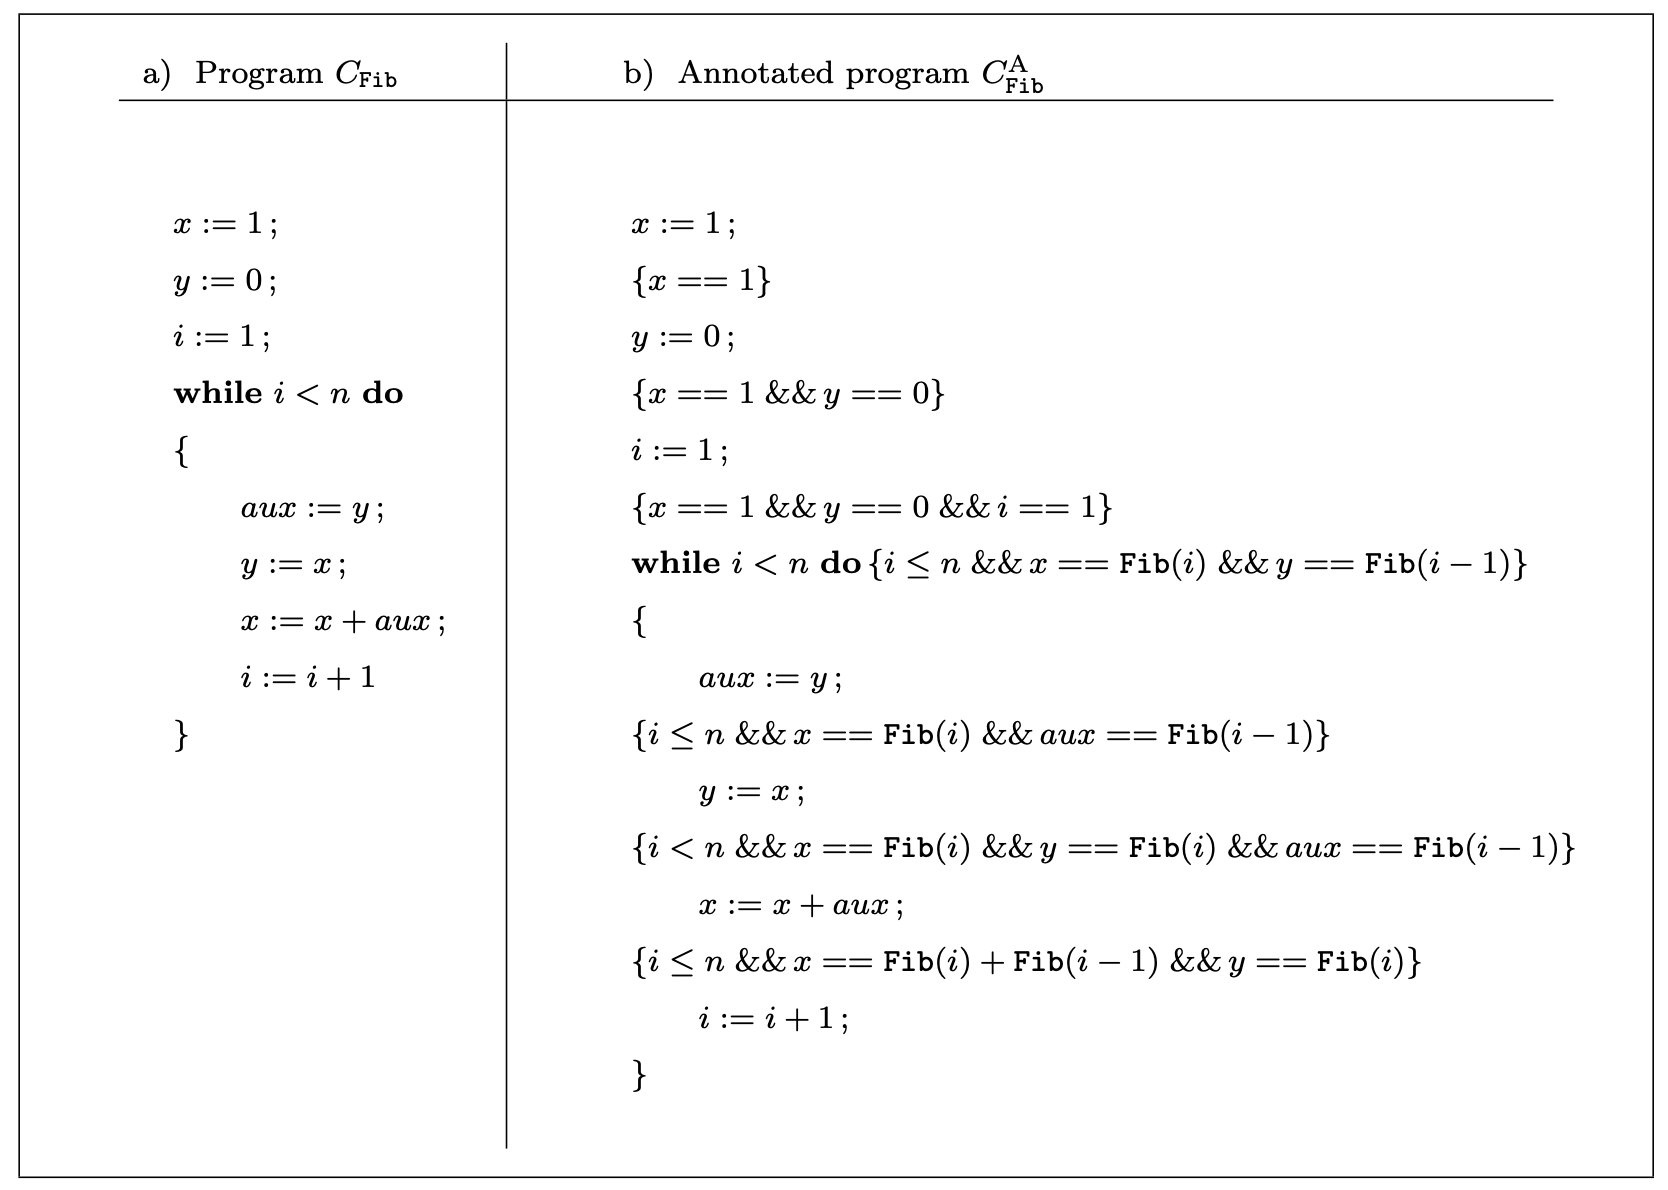
\includegraphics[scale=0.3]{images/fib}
%\end{center}
%\end{slide}
%
%\begin{frame}[fragile]{Extending the annotation to while loops}
%  \begin{block}{The case fo while loops}
%  The new rule for while loops now considers the invariant as an annotation:
%    \begin{prooftree}
%      \AxiomC{$\{B \land I\}\,C\,\{I\}$}
%      \RightLabel{if $P \to I$ and $I \land \neg B \to Q$}
%      \UnaryInfC{$\{P\}\,\kw{while}\;B\;\kw{do}\;\{I\}\;C\;\{Q\}$}
%    \end{prooftree}
%  \end{block}
%\end{frame}

\begin{slide}{Propagation of annotations in code}
 Consider the following code:
\begin{center}

\includegraphics[scale=0.5]{images/ex_code}  
\end{center}
Let us run the first $wprec$ function on this. The actual call to the function will be
$$wprec(aux := y; y := x; x := x + aux, \{x > 10 \land y == 5\})$$ 
\end{slide}

\begin{slide}{Running example - usage of wprec}
\begin{align*}
  \textbf{wprec}(aux := y; y := x; x := x + aux, \{x > 10 \land y == 5\}) & ~=~ \\
  \textbf{wprec}(aux := y,\textbf{wprec}(y := x; x := x + aux, \{x > 10 \land y == 5\})) & ~=~ \\
  \textbf{wprec}(aux := y,\textbf{wprec}(y := x,\textbf{wprec}(x := x + aux, \{x > 10 \land y == 5\}))) & ~=~ \\
  \textbf{wprec}(aux := y,\textbf{wprec}(y := x,\{x > 10 \land y == 5\}[x \mapsto x + aux])) & ~=~ \\
  \textbf{wprec}(aux := y,\textbf{wprec}(y := x,\{x + aux > 10 \land y == 5\})) & ~=~ \\
  \textbf{wprec}(aux := y,\{x + aux > 10 \land y == 5\}[y \mapsto x]) & ~=~ \\
  \textbf{wprec}(aux := y,\{x + aux > 10 \land x == 5\}) & ~=~ \\
  \{x + aux > 10 \land x == 5\}[aux \mapsto y] & ~=~ \\
  \{x + y > 10 \land x == 5\}
\end{align*}
\end{slide}

\begin{slide}{Running example - usage of VC}
\begin{align*}
  \textbf{VC}(\alert{\{x = 5 \land y = 10\}}\,aux := y; y := x; x := x + aux, \alert{\{x > 10 \land y == 5\}}) = \\ \\
  (1)\,\textbf{VC}(\alert{\{x = 5 \land y = 10\}}\,aux := y\,\alert{\{\textbf{wprec}(y := x; x := x + aux, \{x > 10 \land y == 5\})\}})\\
  \cup \\
  (2)\,\textbf{VC}(\alert{\{\textbf{wprec}(y := x; x := x + aux, \{x > 10 \land y == 5\})\}}\,\\y := x; x := x + aux\,\alert{\{x > 10 \land y == 5\}}) =
\end{align*}  
\end{slide}

\begin{slide}{Running example - usage of VC (1)}
\footnotesize{
\begin{align*}
(1)\,\textbf{VC}(\alert{\{x = 5 \land y = 10\}}\,
 aux := y\,
\alert{\{\textbf{wprec}(y := x; x := x + aux, \{x > 10 \land y = 5\})\}})  \\ = \\
\textbf{VC}(\alert{\{x = 5 \land y = 10\}}\,
 aux := y\,
\alert{\{\textbf{wprec}(y := x,\textbf{wprec}(x := x + aux, \{x > 10 \land y = 5\}))\}}) \\ = \\
\textbf{VC}(\alert{\{x = 5 \land y = 10\}}\,
 aux := y\,
 \alert{\{\textbf{wprec}(y := x,\{x > 10 \land y = 5\}[x \mapsto x + aux])\}}) \\ = \\
\textbf{VC}(\alert{\{x = 5 \land y = 10\}}\,
aux := y\,
\alert{\{x > 10 \land y = 5\}[x \mapsto x + aux][y \mapsto x])\}}) \\ = \\
\textbf{VC}(\alert{\{x = 5 \land y = 10\}}\,
aux := y\,
\alert{\{x + aux > 10 \land x = 5\}}) \\ = \\
\{(x = 5 \land y = 10) \to (x + aux > 10 \land x = 5)[aux \to y]\} \\ = \\
\{(x = 5 \land y = 10) \to (x + y > 10 \land x = 5)\}
\end{align*} 
}
\end{slide}

\begin{slide}{Running example - usage of VC (2)}
\footnotesize{
\begin{align*}
(2)\,\textbf{VC}(\alert{\{\textbf{wprec}(y := x; x := x + aux, \{x > 10 \land y = 5\})\}}\,y := x; x := x + aux\,\alert{\{x > 10 \land y = 5\}}) \\ = \\
\textbf{VC}(\alert{\{\textbf{wprec}(y := x,\textbf{wprec}(x := x + aux, \{x > 10 \land y = 5\}))\}}\,y := x; x := x + aux\,\alert{\{x > 10 \land y = 5\}}) \\ = \\
\textbf{VC}(\alert{\{\textbf{wprec}(y := x,\{x > 10 \land y == 5\})[x \mapsto x + aux]\}}\,y := x; x := x + aux\,\alert{\{x > 10 \land y = 5\}}) \\ = \\
\textbf{VC}(\alert{\{x > 10 \land y = 5\}[x \mapsto x + aux][y \mapsto x]}\,y := x; x := x + aux\,\alert{\{x > 10 \land y == 5\}}) \\ = \\
\textbf{VC}(\alert{\{x + aux > 10 \land y = 5\}[y \mapsto x]}\,y := x; x := x + aux\,\alert{\{x > 10 \land y = 5\}}) \\ = \\
\textbf{VC}(\alert{\{x + aux > 10 \land x = 5\}}\,y := x; x := x + aux\,\alert{\{x > 10 \land y = 5\}}) \\ = 
\end{align*}  
}
\end{slide}


\begin{slide}{Running example - usage of VC (2)}
\scriptsize{
\begin{align*}
\textbf{VC}(\alert{\{x + aux > 10 \land x = 5\}}\,
y := x\,
\alert{\{\textbf{wprec}(x := x + aux,\{x > 10 \land y = 5\})\}})\,\\ \cup \\
\textbf{VC}(\alert{\{\textbf{wprec}(x := x + aux,\{x > 10 \land y = 5\})\}}\,
x := x + aux\,
\alert{\{x > 10 \land y = 5\}}) & = \\ \\
\textbf{VC}(\alert{\{x + aux > 10 \land x = 5\}}\,y := x\alert{\{x > 10 \land y = 5\}[x \to x + aux])\}})\,\\\cup \\
\textbf{VC}(\alert{\{x > 10 \land y = 5\}[x \to x + aux])\}}\,x := x + aux\,\alert{\{x > 10 \land y = 5\}}) & = \\ \\
\textbf{VC}(\alert{\{x + aux > 10 \land x = 5\}}\,y := x\,\alert{\{x + aux > 10 \land y = 5\}})\,\\\cup \\
\textbf{VC}(\alert{\{x + aux > 10 \land y = 5\}}\,x := x + aux\,\alert{\{x > 10 \land y = 5\}}) & =
\end{align*}
}  
\end{slide}

\begin{slide}{Running example - usage of VC (2)}
\footnotesize{
\begin{align*}
\{x + aux > 10 \land y = 5 \to (x + aux > 10 \land y = 5)[y \mapsto x]\} \\ \cup \\
\{x + aux > 10 \land y = 5 \to (x > 10 \land y = 5)[x \mapsto x + aux]\} & = \\ \\
\{x + aux > 10 \land y = 5 \to (x + aux > 10 \land x = 5)\} \\ \cup \\
\{x + aux > 10 \land y = 5 \to (x + aux > 10 \land y = 5)\} & =
\end{align*}  
}
\end{slide}

\begin{slide}{Results from propagation}
\begin{center}
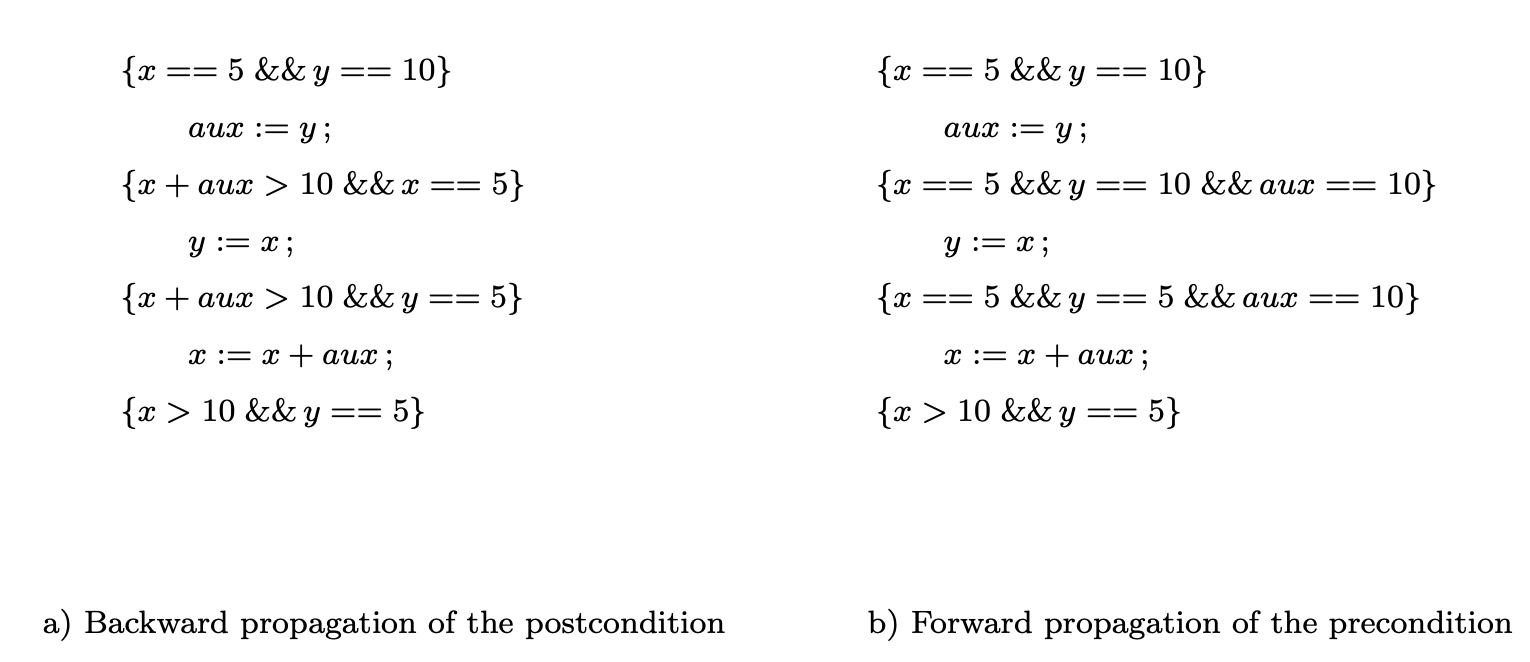
\includegraphics[scale=0.5]{images/ex_code_prop}  
\end{center}
  
\end{slide}

\section*{Weakest Preconditions}

\begin{slide}{Weakest Preconditions}
  \begin{block}{A new look at back propagation of annotations}
  \begin{itemize}
  \item we have seen that back propagating annotations from postconditions works
  \item it can be realised as an algorithm
  \item such algorithm generates the so-called \textbf{weakest preconditions} of an annotated code starting from its postcondition, that is, the weakes conditions that ensure that a program $C$ satisfies the postcondition $Q$ if it terminates, that is $$\{\mathrm{wprec}(C,Q)\}\,C\,\{Q\}$$
  \item if we are able to prove that a precondition $p \to \mathrm{wprec}(C,Q)$ holds, then we can use this weakest precondition generation algorithm to help building the proof tree!
  \end{itemize}
  \end{block}
\end{slide}







%\begin{slide}{While$^{Int}$ with assertions -- Syntax}
%\small
%\begin{align*}
%  x &~\in~ \text{Identifiers}
%  \\
%  n &~\in~ \text{Numerals}
%  \\
%  B &~::=~ \kw{true} ~~|~~ \kw{false} ~~|~~ B \land B ~~|~~ B \lor B ~~|~~ \lnot B ~~|~~ E<E ~~|~~ E=E
%  \tag{boolean-expr}\\
%  E &~::=~ n ~~|~~ x ~~|~~ E+E ~~|~~ E*E ~~|~~ E-E
%  \tag{int-expr}\\
%  C &~::=~ \kw {skip} ~~|~~ C;C ~~|~~ I:=E
%    ~~|~~  \kw{if } B \kw{ then } C\kw{ else }C ~~|~~  \kw{while }B\kw{ do }\alert{\{\phi\}}C
%  \tag{command}\\
%  \alert{\phi} &~::=~ \kw{true} ~~|~~ \kw{false} ~~|~~ x ~~|~~ \phi \land \phi ~~|~~ \phi \lor \phi ~~|~~ \lnot \phi
%    ~~|~~ \alert{\forall x.\phi} ~~|~~ \alert{\exists x.\phi}
%\end{align*}
%
%Assume operators to be left associative.
%\\Use `\{' and `\}' to clarify precedence when necessary.
%
%\end{slide}



\end{document}
